
% !TeX program = lualatex
%%

\documentclass[
	english,
	ruledheaders=section,%Ebene bis zu der die Überschriften mit Linien abgetrennt werden, vgl. DEMO-TUDaPub
	class=report,% Basisdokumentenklasse. Wählt die Korrespondierende KOMA-Script Klasse
	thesis={type=master},% Dokumententyp Thesis, für Dissertationen siehe die Demo-Datei DEMO-TUDaPhd
	accentcolor=1c,% Auswahl der Akzentfarbe
	custommargins=true,% Ränder werden mithilfe von typearea automatisch berechnet
	marginpar=false,% Kopfzeile und Fußzeile erstrecken sich nicht über die Randnotizspalte
	%BCOR=5mm,%Bindekorrektur, falls notwendig
	parskip=half-,%Absatzkennzeichnung durch Abstand vgl. KOMA-Script
	fontsize=11pt,%Basisschriftgröße laut Corporate Design ist mit 9pt häufig zu klein
%	logofile=example-image, %Falls die Logo Dateien nicht vorliegen
]{tudapub}


% Der folgende Block ist nur bei pdfTeX auf Versionen vor April 2018 notwendig
\usepackage{iftex}
\ifPDFTeX
	\usepackage[utf8]{inputenc}%kompatibilität mit TeX Versionen vor April 2018
\fi

%%%%%%%%%%%%%%%%%%%
%Sprachanpassung & Verbesserte Trennregeln
%%%%%%%%%%%%%%%%%%%
\usepackage[english, main=english]{babel}
\usepackage[autostyle]{csquotes}% Anführungszeichen vereinfacht

% Falls mit pdflatex kompiliert wird, wird microtype automatisch geladen, in diesem Fall muss diese Zeile entfernt werden, und falls weiter Optionen hinzugefügt werden sollen, muss dies über
% \PassOptionsToPackage{Optionen}{microtype}
% vor \documentclass hinzugefügt werden.
\usepackage{microtype}
\usepackage{todonotes}
%%%%%%%%%%%%%%%%%%%
%Literaturverzeichnis
%%%%%%%%%%%%%%%%%%%
\usepackage{biblatex}   % Literaturverzeichnis
\usepackage[utf8]{inputenc}
\usepackage[acronym]{glossaries}
\bibliography{DEMO-TUDaBibliography}


%%%%%%%%%%%%%%%%%%%
%Paketvorschläge Tabellen
%%%%%%%%%%%%%%%%%%%
%\usepackage{array}     % Basispaket für Tabellenkonfiguration, wird von den folgenden automatisch geladen
\usepackage{tabularx}   % Tabellen, die sich automatisch der Breite anpassen
%\usepackage{longtable} % Mehrseitige Tabellen
%\usepackage{xltabular} % Mehrseitige Tabellen mit anpassbarer Breite
\usepackage{booktabs}   % Verbesserte Möglichkeiten für Tabellenlayout über horizontale Linien

%%%%%%%%%%%%%%%%%%%
%Paketvorschläge Mathematik
%%%%%%%%%%%%%%%%%%%
\usepackage{mathtools} % erweiterte Fassung von amsmath
\usepackage{amssymb}   % erweiterter Zeichensatz
\usepackage{siunitx}   % Einheiten
\usepackage{amsmath}


\usepackage{xcolor}
\usepackage{listings}
\usepackage{xparse}


\usepackage{tikz}
\usepackage{geometry}
\usepackage[export]{adjustbox}



%Formatierungen für Beispiele in diesem Dokument. Im Allgemeinen nicht notwendig!
\let\file\texttt
\let\code\texttt
\let\tbs\textbackslash
\let\pck\textsf
\let\cls\textsf

\usepackage{pifont}% Zapf-Dingbats Symbole
\usepackage{layouts}
\newcommand*{\FeatureTrue}{\ding{52}}
\newcommand*{\FeatureFalse}{\ding{56}}




\begin{document}

\Metadata{
	title=Towards direct numerical simulations of mesopore imbibition, using a phase-field approach in OpenFOAM,
	author=Jan Kröger
}

\title{Towards direct numerical simulations of mesopore imbibition, using a phase-field approach in OpenFOAM}
%\subtitle{\LaTeX{} using TU Darmstadt's Corporate Design}
\author[J. Kröger]{Jan Kröger}%optionales Argument ist die Signatur,
\birthplace{Köln}%Geburtsort, bei Dissertationen zwingend notwendig
\reviewer{Professor Dieter Bothe \and Holger Marschall}%Gutachter

%Diese Felder werden untereinander auf der Titelseite platziert.
%\department ist eine notwendige Angabe, siehe auch dem Abschnitt `Abweichung von den Vorgaben für die Titelseite'
\department{math} % Das Kürzel wird automatisch ersetzt und als Studienfach gewählt, siehe Liste der Kürzel im Dokument.
\institute{Fachbereich Mathematik}
\group{Computational Multiphase Flow}

\submissiondate{\today}
\examdate{\today}

% Hinweis zur Lizenz:
% TUDa-CI verwendet momentan die Lizenz CC BY-NC-ND 2.0 DE als Voreinstellung.
% Die TU Darmstadt hat jedoch die Empfehlung von dieser auf die liberalere
% CC BY 4.0 geändert. Diese erlaubt eine Verwendung bearbeiteter Versionen und
% die kommerzielle Nutzung.
% TUDa-CI wird im nächsten größeren Release ebenfalls diese Anpassung vornehmen.
% Aus diesem Grund wird empfohlen die Lizenz manuell auszuwählen.
%\tuprints{urn=XXXXX,printid=XXXX,year=2022,license=cc-by-4.0}
% To see further information on the license option in English, remove the license= key and pay attention to the warning & help message.

% \dedication{Für alle, die \TeX{} nutzen.}

%%%%%%%%%%%%%%%%%\maketitle

\affidavit
% Es gibt mit Version 3.20 die Möglichkeit ein Bild als Signatur einzubinden.
% TUDa-CI kann nicht garantieren, dass dies zulässig ist oder eine eigenhändige Unterschrift ersetzt.
% Dies ist durch Studierende vor der Verwendung abzuklären.
% Die Verwendung funktioniert so:
%\affidavit[signature-image={\includegraphics[width=\width,height=1cm]{example-image}}, <hier können andere Optionen zusätzlich stehen>]

\tableofcontents
\listoftodos





\chapter{Introduction}
\label{chap: Introduction}
Many everyday phenomena that we observe are, contrary to expectations, not yet fully understood. This does not mean that they are not utilized in a variety of technical devices. In the case of wetting, we encounter many different things in everyday life, such as a drop on a window pane that seems to slide down randomly, or the sleeve of a sweater that seems to soak up water when washing hands.

Nature has a head start in this effect and has produced creatures that can walk on water because they take advantage of the water's surface tension. The flora also uses surface tension, whether it's trees that wouldn't reach the size we know without the capillary effect, or the lotus flower, which, with its water-repellent (hydrophobic) surface, ensures that water rolls off and takes dirt with it in the process.

Porous media, through their use in oxygenators, became lifesavers during the Corona pandemic by reoxygenating blood. The potential applications and necessities of this phenomenon could be demonstrated with many more examples. This work aims to describe the dynamics of capillary rise through simulations. A porous medium can be simplified as a collection of many small tubes. Insights from these small tubes can then be extrapolated to determine the behavior of the porous medium. Therefore, experiments with both porous media and individual capillaries are of great interest to understand how the rise in the capillary is designed. Simulations of these processes are also increasingly being carried out, as they have the advantage of fixing certain relevant material properties to examine their influence, or to look into areas that would not be possible with a conventional experimental setup.

In this work, the rise of a liquid column (water) in a capillary is investigated. Specifically, for a two-phase system, the area around the interface in the water phase is examined, and how dissipative processes in this region influence the rise of the water column. Possible phase changes (evaporation, boiling, condensation, etc.) are not taken into account. An isothermal and isobaric system is also assumed. All fluids treated are Newtonian, and the flow can be assumed to be Poiseuille flow. Furthermore, newly implemented boundary conditions of the used solver, which are supposed to better represent the behavior of the contact line and contact angle, will also be checked. 

This work will first discuss important findings in the description of capillary rise, the contact line, and the simulation of such problems with phase field methods in Chapter \ref{chap: BibliographyReview}. This is followed by an overview of the important influencing factors of wetting and their influence on the topics discussed in Chapter \ref{chap: wettingTheory}. Chapter \ref{chap: PhaseFieldMethod} provides an introduction to the phase field method and how it is implemented to simulate such problems. Chapter \ref{chap: Validation} shows that the solver used has already shown in many other simulations that it produces correct results and is applicable to these problems. Validation of the geometries used here is not possible due to their size, as they have a radius of 3 nm. It is not currently known that there are experiments that provide reliable results with a constant cross-section and such small radii. Subsequently, Chapter \ref{chap: CaseSetup} describes the setup of the simulations with descriptions of the geometry, material properties used, and solver settings. Finally, the results are discussed in Chapter \todo{ADD CHAPTER}, and an outlook for upcoming investigations is given in Chapter \todo{ADD CHAPTER}.

The solver used here is \texttt{phaseFieldFoam}, which is an extension of the open-source environment \texttt{OpenFOAM-extend}. The version used of \texttt{OpenFOAM-extend} is 5.0, and the version of the solver is still in development. The further development and maintenance of the solver are carried out through a cooperation between KIT (Karlsruhe Institute of Technology) and TU Darmstadt, especially by Dr.-Ing. Xuan Cai and Dr.-Ing. Holger Marschall. The simulations for this research were conducted on the Lichtenberg high-performance computer of the TU Darmstadt.




\todo[inline]{Here a introduction, but probably only after the most is done and the layout of the thesis is set.}

The dynamics of a rising fluid in the capillary is the subject of many processes. In nature, for example, trees would not be able to grow as high as they do without the capillary effect, and in technology many processes with a porous medium exist. Porous media can be simplified as many small tubes through which a fluid travels. Therefore, this process has long been of great interest in science and yet there are many uncertainties in the description of the dynamics.   

The Lucas Washburn equation, introduced in 1921 \cite{lucas_ueber_1918, washburn_dynamics_1921}, attempts to describe the height of the propagating fluid column as a function of time. This equation is sufficiently accurate for many applications.   
  
However, due to the assumptions made in the derivation of the equation, it is clear that it cannot be applied to every problem. Therefore, there are many approaches to adapt this equation to problems and simply maintain the behaviour of the equation. 

It is shown, that the Lucas Washburn equation has its problems in early stages of the imbibition\cite{bosanquet_lv_1923, quere_inertial_1997}\todo{check if quere1997 is also a source. Probably talked about that. Maybe even Washburn talked about that? }, due to the undefined behaviour for $t=0$ and neglecting the inertia of the fluid. 

The early stages of the imbibition process is yet to be understood and in this work we show how the different forces are acting on the meniscus for small time steps with a simulation of the such a problem. This simulations are done with the open source framework of foam extend, which is a fork of open foam. Here the department of mathmatics of the TU Darmstadt and the KIT developed a solver for a phase field approach. \todo{rework this regment.}

The developed solver phaseFieldFoam is maintained and developed by the department of MMA at the Tu darmstadt and ... KIT. It is using the Phase field approach to solve the Navier Stokes Equations (NSE).

In this work, first the attempts to describe the imbibition of a fluid in a capillay, especially for the early stages and small capillaies are discussed\todo{ref chapter}. Followed by the work, which has been done to simulate such problems with the phase field approach\todo{ref chapter}. Important interrelationships and derivations of the process of wetting is discussed, again followed by the equivalent numerical relations\todo{ref to both chapters}. How the simulations are setup and the results are in the chapers \todo{chapter} and \todo{chapter}.  


Lucas needed to prewet the tube to get the results he predicted 

In this work 

%\chapter{Bibliography Review}
%\label{chap: BibliographyReview}
%\input{bibliographyReview}

\chapter{Wetting Theory}
\label{chap: wettingTheory}
The wetting theory describes the interaction of fluids with solid surfaces. Many processes in nature, as well as in technology, are affected by this phenomenon. In this work, the focus is on the wetting properties in capillaries, which are often used as a simplification for understanding porous media or in other processes, such as the fact that trees would not be as tall as they are today without this effect. 

First, an overview of some types of wetting is presented \todo{ref}, and the concepts of contact angle and contact line are introduced. Subsequently, the surface tension \todo{ref} and its role in wetting are discussed. Since this work considers the dynamic rise of a water column in a capillary, the dynamic contact angle is also examined in Chapter \todo{ref chapter}, followed by a description of the capillary effect \todo{ref} and its significance for the rise of a fluid in a capillary. \todo{rework}

\section{Surface Tension}
\label{sec: Wetting_SurfaceTension}
Surface tension plays a significant role in the wetting of surfaces or in capillary rise. Therefore, it is essential to first clarify what surface tension is. In general, surface tension is a proportionality constant that depends on temperature, pressure, and the phases involved but is independent of the surface \cite{buttPhysicsChemistryInterfaces}. The interface separates the phases and can be interpreted differently. \todo{possibly ref to corresponding chapters here.}
On a molecular level, molecules attract each other (cohesion). The interaction between two phases is called adhesion. In the case of the interaction between a liquid and a solid, adhesion can usually be neglected. In Figure \ref{fig: WettingTheory_SurfaceTensionMolecules}, a water droplet surrounded by air is illustrated on the left. The black outer line thus represents the interface between the droplet and the air. If one now magnifies the transition area down to the molecular level (red area), one obtains the schematic representation on the right side. The blue circles are simplified representations of the water molecules, and the gray ones represent the surrounding air. Here, it is evident how, at the interface, the water molecules are no longer surrounded only by other water molecules, which is energetically unfavorable. However, since the system strives to transition into an energetically favorable state, it attempts to minimize the number of molecules lying at the interface \cite{buttPhysicsChemistryInterfaces}.

\begin{figure}[h]
    \centering
    \includegraphics[width=.9\textwidth]{Pictures/moleculesAhesionCohesion_Wetting.pdf}
    \caption{Schematic of interacting molecules in a liquid droplet and its interaction with a vapor}
    \label{fig: WettingTheory_SurfaceTensionMolecules}
\end{figure}
To increase the surface area, molecules must be transported to the surface, and energy must be supplied to the system. Therefore, surface tension is also interpreted as the necessary energy required to carry a molecule to the surface.
\begin{equation}
    dE = \sigma \cdot dA
\end{equation}
with \(dE\) as the supplied energy and \(dA\) as the change in surface area.


\section{Wetting Phenomenon}
Despite the fact that the wetting of droplets is not considered in this work, it is appropriate to describe the fundamentals of wetting using this example. The concepts are the same, and many initial studies are based on this example.

In the case where the system is in equilibrium, Young \cite{youngIIIEssayCohesion1805} derived an equation relating surface tensions to the contact angle:
\begin{equation}
    \sigma_{\mathrm{LV}} \cdot \cos\theta_{\mathrm{e}} = \sigma_{\mathrm{SV}}-\sigma_{\mathrm{SL}}
    \label{eq: YoungsEQ}
\end{equation}
Where $\sigma_{\mathrm{LV}}$ is the surface tension between the liquid and the gas, $\sigma_{\mathrm{SV}}$ is from the solid to the gas, and $\sigma_{\mathrm{SL}}$ is between the solid and the liquid (see Figure \ref{fig: YoungsLaw_ThreePhaseContactLine}).
\begin{figure}[h]
    \centering
    \includegraphics[width=.9\textwidth]{Pictures/YoungsLaw.pdf}
    \caption{Three Phase Contact Line}
    \label{fig: YoungsLaw_ThreePhaseContactLine}
\end{figure}
If $(\sigma_{\mathrm{SV}}>\sigma_{\mathrm{SL}})$ holds true, a contact angle less than $90^{\circ}$ follows; otherwise, $90^{\circ}\leq \theta_{\mathrm{e}}<180^{\circ}$. In the case where $\sigma_{\mathrm{SV}}=\sigma_{\mathrm{SL}}+\sigma_{\mathrm{LV}}$, complete wetting of the surface occurs \cite{buttPhysicsChemistryInterfaces}.

When a droplet impacts a solid surface, different states can arise depending on the fluid-solid combination. At the point where the interface of the two fluids (droplet and surrounding fluid) meets the solid surface, the contact line is formed (see \ref{fig: YoungsLaw_ThreePhaseContactLine}; red line). Depending on the fluid-fluid-solid combination, a contact angle $\theta_{\mathrm{e}}$ is established, where the suffix $e$ stands for equilibrium. In the case of complete wetting, the fluid spreads over the entire surface (see Figure \ref{fig: WettingTheory_WettingOfSurface} a)). This effect, however, is challenging to reproduce as it can be hindered by surface irregularities \cite{buttPhysicsChemistryInterfaces}. As seen in Figure \ref{fig: WettingTheory_WettingOfSurface}(b-d)), states where a droplet forms on the surface are further subdivided. For a contact angle $\theta_{\mathrm{e}}<90^{\circ}$, it is termed hydrophilic (see \ref{fig: WettingTheory_WettingOfSurface}b)), for $\theta_{\mathrm{e}}>90^{\circ}$ it's hydrophobic (see \ref{fig: WettingTheory_WettingOfSurface}c)), and for a contact angle $\theta_{\mathrm{e}}>120^{\circ}$, it's superhydrophobic surfaces (see \ref{fig: WettingTheory_WettingOfSurface}d)). Developing superhydrophobic surfaces is also challenging.
\begin{figure}[h]
    \centering
    \includegraphics[width=.95\textwidth]{Pictures/DropletsAndWetting.pdf}
    \caption{Wetting of a surface}
    \label{fig: WettingTheory_WettingOfSurface}
\end{figure}
To curve the surface of the liquid, a pressure difference must exist. In the case of a sphere, Young and Laplace developed a relationship for the pressure difference in terms of the surface tension and radius as:
\begin{equation}
\label{eq: YoungLaplaceEQ}
    P_{\mathrm{i}} - P_{\mathrm{o}} = \Delta P =  \frac{2\sigma}{R}
\end{equation}
With $\Delta P$ being the pressure difference at the interface, $P_{\mathrm{i}}$ as the pressure inside the droplet, $P_{\mathrm{o}}$ the ambient pressure, and $R$ as the radius of the sphere. For a derivation, refer to \cite{buttPhysicsChemistryInterfaces}.


\subsection{Dynamic Weting}
So far, only states have been considered that observe systems in equilibrium. Typically, however, the contact line is in motion. When the contact line is moving, the contact angle (dynamic contact angle $\theta_{\mathrm{D}}$) differs from that in the equilibrium state \cite{blake2006PhysicsMovingWetting}. To describe the dynamics of the contact line, the dynamic contact angle, the relative speed of the contact line, and the equilibrium contact angle are required \cite{mohammadkarim2022ReviewPhysicsMoving, blake2006PhysicsMovingWetting, cox1986DynamicsSpreadingLiquids,huh1971HydrodynamicModelSteady,voinovHydrodynamicsWetting1977}. However, describing the contact line is challenging due to the fact that the microscopic level affects the macroscopic level.

In Figure \ref{fig: HDT_MKT_comp}, various views of the contact line are illustrated. The red circle in \textit{a)} points to the area considered in the picture next to it and can be understood as a magnifying glass. If we enlarge the area in \textit{a)}, we see the interpretation of the contact line from the perspective of the hydrodynamic theory, with a microscopic contact angle $\theta_{\mathrm{m}}$ and the dynamic contact angle $\theta_{\mathrm{D}}$ (Figure \ref{fig: HDT_MKT_comp} \textit{b)}). Focusing again on the contact line, we see the interpretation of the molecular kinetic theory (Figure \ref{fig: HDT_MKT_comp} \textit{c)}). The illustrated points are intended to represent molecules in a simplified form.




\begin{figure}[h]
    \centering
    \includegraphics[width=.95\textwidth]{Pictures/ContactAngles_HDT_MKT.pdf}
    \caption{Hydrodynamic and Molecular Kinetic description of the Contact angle. Figure b) corresponds to the area circled in red in a), and c) to the area from image b).}
    \label{fig: HDT_MKT_comp}
\end{figure}

\paragraph{Hydrodynamic Theory}
\label{paragraph: hydrodynTheory}
The hydrodynamic approach solves the physics of the flow using the Navier-Stokes equations but encounters a singularity at the contact line when a sticking condition is applied \cite{huh1971HydrodynamicModelSteady}. To address this issue, either the sticking condition near the wall was relaxed or the solution was truncated at the molecular level \cite{blake2006PhysicsMovingWetting}. In both cases, a small capillary number is assumed, which means that far from the contact line, the interface assumes its equilibrium shape.

Voinov \cite{voinovHydrodynamicsWetting1977} derived a description of the contact line for a spreading droplet depending on the capillary number. A generalized version was developed by Cox \cite{cox1986DynamicsSpreadingLiquids} with some correction terms \cite{carlsonCapillarityDynamicWetting2012,blake2006PhysicsMovingWetting}. Thus, the dynamic contact angle for $\theta_{\mathrm{D}} \leq 3/4 \pi$ is given by
\begin{equation}
    \label{eq: Cox-Voinov}
    \theta_D^3-\theta_m^3= 9 Ca \ln\left(\frac{L}{L_m}\right) = 9 \frac{\mu u}{\sigma}\ln\left(\frac{L}{L_m}\right)
\end{equation}
With $L$ as the macroscopic path length and $L_{\mathrm{m}}$ as the microscopic path length. Assuming that the interface assumes its equilibrium shape far away, $\theta_{\mathrm{m}} = \theta_{\mathrm{e}}$. However, Voinov himself already pointed out that $\theta_{\mathrm{m}}$ could also depend on the speed \cite{voinovHydrodynamicsWetting1977,blake2006PhysicsMovingWetting,lacisNanoscaleShearedDroplet2022}.


\paragraph{Molecular Kinetic Theory}
The Molecular Kinetic Model describes the movement of the contact line with a statistical description of the molecular movement at the contact line \cite{blake1969KineticsDisplacement}. 
In contrast to the hydrodynamic model, the molecular processes at the contact line influence those of the larger scales. In this view, the molecules at the contact line jump back and forth to adsorption sites on the solid substrate. The speed of the contact line is determined by multiplying the difference between the forward and backward jumps by a jump distance $\lambda$. This results in the description
\begin{equation}
    u=2\lambda\kappa_{0}\sinh\left(\frac{\sigma\left(\cos\theta_{\mathrm{e}}-\cos\theta_{\mathrm{D}}\right)}{2nk_{\mathrm{B}}T}\right).
\end{equation}
Where $n$ is the number of adsorption sites per unit area, $k_0$ is a characteristic frequency, $k_{\mathrm{B}}$ is the Boltzmann constant, and $T$ is the temperature.
If the system is in equilibrium, the forward and backward jumping is balanced, and the contact line comes to a standstill \cite{carlson2011DissipationRapidDynamic,blake2006PhysicsMovingWetting}. However, a problem with this view is that this model is more qualitative and computationally intensive \cite{mohammadkarim2022ReviewPhysicsMoving}.








\subsection{Capillary Rise}
\label{sec: capillaryRise}
A capillary is a very thin tube in which, due to surface effects, a liquid rises or falls without external force. In \ref{fig: classicCapillary}, a capillary with an already risen liquid column is shown. The well-known surface tensions are also marked at their respective locations, as well as the essential geometric parameters, such as diameter ($2R$) or height of the resulting meniscus $z$. The resulting contact angle after reaching equilibrium, $\theta_{\mathrm{e}}$, is also shown. The system in this representation is also subject to gravitational forces.

\begin{figure}[h]
    \centering
    \includegraphics[width=.95\textwidth]{Pictures/classicCapillary.pdf}
    \caption{Schematic representation of a capillary in a liquid after it has penetrated the capillary.}
    \label{fig: classicCapillary}
\end{figure}

In this work, such a system is used. However, further conditions apply. It is assumed that the system is isobaric, isothermal, and the liquid is Newtonian. Furthermore, it is assumed that while the water column rises in the capillary, a Poiseuille flow is present and no phase change occurs. It is also assumed that the viscosity of the gas phase is negligible. With these assumptions and boundary conditions, the Newtonian dynamics in a capillary can be described as a balance between the inertial forces and the sum of the capillary forces, viscous forces, and hydrostatic forces \cite{fricke2023AnalyticalStudyCapillary}:

\begin{equation}
\label{eq: NewtonBalanceForcesOnly}
    \frac{d}{dt}M(z,\dot{z}) = F_{\mathrm{w}} - F_{\eta} - F_{\mathrm{g}}
\end{equation}

With $M(z,\dot{z}) = \pi r^2 \rho z \dot{z}$ as the moment, $F_{\mathrm{g}} = \pi r^2 \rho g z$ as the gravitational force, and $F_{\eta}$ as the viscous resistance, which results from the assumption of the average velocity and the existing Poiseuille flow to $F_{\eta}=8\pi\eta z \dot{z}$. With $\dot{z}$ as the average velocity. The capillary forces result from the previous description of the surface tension and the change in the surface of the meniscus with a change in the current height:

\begin{equation}
    F_{\mathrm{w}}=\sigma \frac{dA}{dz} = \sigma 2\pi r
\end{equation}

The surface tension $\sigma$ here is the increase in surface energy due to the wetting of the solid wall of the capillary. Thus, $\sigma = \sigma_{\mathrm{SV}}- \sigma_{\mathrm{SL}}$. This description is already known from the Young equation (\ref{eq: YoungsEQ}). Thus, after inserting for the capillary forces:

\begin{equation}
    F_W = \sigma_{\mathrm{LV}} \cdot \cos \theta_{\mathrm{e}} 2\pi r.
\end{equation}

Thus, for equation \ref{eq: NewtonBalanceForcesOnly} after insertion \cite{fricke2023AnalyticalStudyCapillary}:

\begin{equation}
\label{eq: NewtonDynCapillary}
    \pi r^2 \rho \frac{d}{dt} (z \dot{z}) = \sigma_{\mathrm{LV}} \cdot \cos \theta_{\mathrm{e}} 2\pi r-8\pi\eta z \dot{z}-\pi r^2 \rho g z.
\end{equation}

Early descriptions by Bell and Cameron \cite{bell1906FlowLiquidsCapillary} did not describe the rise dynamics based on equation \ref{eq: NewtonDynCapillary}. They developed the rise dynamics from experiments according to:

\begin{equation}
    z(t)^n = K\cdot t.
\end{equation}

Both $n$ and $K$ are temperature-dependent constants. In 1918, Lucas \cite{lucas1918UeberZeitgesetzKapillaren} and in 1921, Washburn \cite{washburn1921DynamicsCapillaryFlow} derived the Lucas Washburn equation by neglecting the inertial and gravitational terms:

\begin{equation}
\label{eq: LW-Eq}
    z(t) = \sqrt{\frac{r\sigma\cos\theta_{\mathrm{e}}}{2\eta}t}
\end{equation}

With this, they independently developed an equation with which the capillary rise can be described based on material values and measurements. Therefore, it gained popularity over the years. Due to the neglect of individual terms and simplifications in the system, however, this equation is not always precise for several reasons. Washburn himself pointed out that to meet the prediction of the equation, he had to set up the experiments in such a way that the capillary was prewetted. Therefore, adjustments to this equation were made for various problems \cite{dimitrov2007CapillaryRiseNanopores, heiranian2022ModifiedLucasWashburnTheory,cai2021LucasWashburnEquationBased,fries2008AnalyticSolutionCapillary,fricke2023AnalyticalStudyCapillary,delannoy2019DualRoleViscosity,martic2002MolecularDynamicsSimulation}. Wu et al. \cite{wu2017CapillaryRiseValidity} examined several models and compared them with experiments. In these, however, it is always assumed that the height of the meniscus increases according to $z(t)\sim \sqrt{t}$ as well.

Bosanquet \cite{bosanquet1923LVFlowLiquids} hinted in his 1923 paper that equation \ref{eq: LW-Eq} would lead to unphysical behavior for $t\xrightarrow{}0$ and also developed an equation that retained this problem but now also included inertia and can give a better prediction of the rise for early times of imbibition, but also fails for small capillary \cite{chen2023InvestigatingValidityBosanquet}. 

Siegel \cite{siegel1961TransientCapillaryRise} studied the rise behavior under microgravity and found a linear growth. However, he did not reach the Lucas-Washburn regime. Zhmud et al. \cite{zhmud2000DynamicsCapillaryRise} also pointed out the problems for times near $0$ from equation \ref{eq: LW-Eq} and described a quadratic relationship for the times when the fluid is drawn into the capillary, followed by the known Lucas-Washburn regime.

Dreyer et al. \cite{dreyer1994CapillaryRiseLiquid} studied parallel plates under microgravity and divided the rise of the meniscus into three regions. Starting with a quadratic growth, followed by a linear region, and finally the Lucas-Washburn growth. Quéré \cite{quere1997InertialCapillarity} showed a linear growth at the beginning by assuming that in this case only inertia plays a role. Stange \cite{stange2003CapillaryDrivenFlow} confirmed the three regions of Dreyer et al. \cite{dreyer1994CapillaryRiseLiquid} and derived dimensionless equations to develop transition times.

Fries et al. \cite{fries2008TransitionInertialViscous} divided the growth area into areas where different forces act. In the beginning, inertia dominates, followed by a transition area where the viscous forces take over until they finally dominate. They also developed dimensionless times at which the transition takes place.

At the point where the viscous friction and the effects of inertia or dynamic contact angle are equal, Quéré \cite{quere1997InertialCapillarity} and Fries et al. \cite{fries2008TransitionInertialViscous} defined the characteristic penetration length:
\begin{equation}
    \label{eq: charLength}
    l_{\mathrm{c}} \propto r \sqrt{\frac{r\rho \sigma}{\mu^2}}
\end{equation}
Dellanoy et al. \cite{delannoy2019DualRoleViscosity} focused on early times and studied viscous fluids, confirming the influence of pre-wetting the capillary, as already mentioned by Washburn \cite{washburn1921DynamicsCapillaryFlow}. They also showed a deviation from the Lucas-Washburn regime at early times. They attributed this deviation to local viscous dissipation in the wedge region, rather than a global dissipation as assumed by Lucas and Washburn. Regarding the dynamic contact angle, they showed that the characteristic penetration length (cf. Equation \ref{eq: charLength}) is calculated as:
\begin{equation}
    l_{\mathrm{c}} \propto r \ln\left(\frac{r}{l_{\mathrm{m}}}\right)
\end{equation}

With $l_m$ being the microscopic length that compensates for the singularity of the contact line \cite{cox1986DynamicsSpreadingLiquids}. They further assumed that once $l_c$ is reached, the transition to the Lucas-Washburn regime occurs.

Ruiz-Gutiérrez et al. \cite{ruiz-gutierrez2022LongCrossoverDynamics} contradicted this statement in their work, showing that this transition takes longer. They argue that the effects of inertia and dynamic contact angle do not decay exponentially. 

To account for this, they expanded Equation \ref{eq: NewtonDynCapillary} for problems with a moving interface by introducing:
\begin{equation}
    f(\dot{z}) \equiv \frac{\cos\theta_{\mathrm{m}}-\cos\theta_D(\dot{z})}{\cos\theta_{\mathrm{m}}} 
\end{equation}
With the assumption that for $u>0$ from Equation \ref{eq: Cox-Voinov}, $\theta_{\mathrm{D}} > \theta_{\mathrm{m}}$ holds true, this function disappears for $\theta_{\mathrm{D}} \rightarrow \theta_{\mathrm{m}}$. 

Now, considering the moving system, Equation \ref{eq: NewtonDynCapillary} for the case studied in this work becomes:
\begin{equation}
    \pi r^{2}\rho z \frac{du}{dt}= 2\pi r\sigma \cos\theta_{\mathrm{m}}+\pi r^{2}\rho gz-8\pi \sigma z \dot{z} -2\pi r \sigma \cos \theta_{\mathrm{m}}f
\end{equation}
With the first two terms as driving forces and the last two as resistance forces. The last term has been added and acts as a correction for the fact that the dynamic contact angle does not correspond to the macroscopic contact angle.

Subsequently, dimensionless quantities were introduced, and four cases were defined. Two each with a large and small Laplace number, or a large and small ratio of length scales. With the quantities used in this work, case three from Ruiz-Gutiérrez et al. \cite{ruiz-gutierrez2022LongCrossoverDynamics} should apply. They predict that the quadratic regime will not occur, and the rise will begin with a linear region, eventually transitioning to the Lucas-Washburn regime.


\todo[inline]{maybe use this eq instead of shorted one?}
\begin{equation}
    \pi r^2\rho l\frac{\mathrm{d}u}{\mathrm{d}t}=2\pi r\gamma\cos\theta_{\mathrm{a}}+\pi r^2\rho gh-8\pi\mu lu-\frac{3}{2}\pi r^2\rho u^2-2\pi r\gamma\cos\theta_{\mathrm{a}}f
\end{equation}


\section{Simulating the Wetting Processes}
Simulating a two-phase flow can be achieved through several methods. Common approaches include the \texttt{Volume-of-Fluid} and the \texttt{Level-Set} methods. Both methods use a sharp interface and are based on the Hydrodynamic Theory from Chapter \ref{paragraph: hydrodynTheory}. Moreover, they are \textit{interface capturing} methods, so they don't require recalculating the computational grid over the simulation period. Other methods that follow the interface (\textit{interface tracking}) are also possible. One of the major drawbacks of these methods is that the moving contact line, when using the adhesion condition, depends on models \cite{carlsonCapillarityDynamicWetting2012}. Additionally, calculating the surface tension can pose a challenge. This requires computing the curvature of the surface, which can lead to relatively high numerical errors \cite{jamshidi2019SuitabilityPhasefieldAlgebraic,hagg2019DirekteNumerischeSimulation}.

The Lattice-Boltzmann Method uses collision models to describe fluid behavior. Surface tensions can be considered through modifications. There are approaches that are promising and some are comparable to the phase-field method. However, one of the biggest challenges is the limitation of density or viscosity ratios. In this work, the fluids have significantly different densities with a ratio of $1000$. According to \cite{chenCriticalReviewPseudopotential2014}, the Lattice-Boltzmann Method is limited to ratios of $\mathcal{O}(10)$ and can lead to instabilities otherwise.

Another frequently used method is \texttt{Molecular Dynamic} simulations. Since individual molecules are simulated in this case, this method is only applicable to geometrically and temporally small problems without driving computational costs too high. Therefore, \texttt{Molecular Dynamic} simulations are often used for comparison or to study only small problems (\cite{datta2023EarlyStageLiquidInfiltration,lacisNanoscaleShearedDroplet2022,martic2002MolecularDynamicsSimulation,dimitrov2007CapillaryRiseNanopores}).

The method used in this work is the \texttt{phase-field} method. This method models two or even multi-phase flow through the system's free energy. A more detailed description of this method and the simulations already carried out is provided in Chapter \ref{chap: PhaseFieldMethod}. \todo[inline]{Elaborate or maybe move the entire section to phase field? Or perhaps case setup with a reasoning why phase field?}



\chapter{Phase Field Method}
\label{chap: PhaseFieldMethod}
The phase field method, rooted in system thermodynamics, offers a solution for an interface with a finite thickness, an idea originating from van der Waals in 1893 \cite{vanderwaals1979ThermodynamicTheoryCapillarity}. This method models the free energy of the system and can derive a phase field method for interfacial dynamics. It offers several advantages, such as mass conservation, contact line motion, and adherence to thermodynamic laws. In contrast to the hydrodynamic theory, the contact line moves through interfacial diffusion. However, there are concerns about its validity in modeling macroscopic contact line motion, especially regarding the sharp-interface limit. Despite these concerns, meaningful results have been predicted on the macro scale that align with hydrodynamic theory and experimental observations\cite{yue2010SharpinterfaceLimitCahn,yue2011CanDiffuseinterfaceModels,carlson2011DissipationRapidDynamic}.


Phase field simulations for macroscopic wetting typically rely on the Cahn-Hilliard equations. For slow wetting phenomena, the phase field theory has been both analytically \cite{jacqmin2000ContactlineDynamicsDiffuse} and numerically \cite{yue2011CanDiffuseinterfaceModels,yue2010SharpinterfaceLimitCahn} proven to capture such wetting physics. However, for rapid spreading of water drops, the assumption of local equilibrium may not hold. Some studies have introduced a boundary condition for wetting far from equilibrium, introducing a parameter that controls the relaxation towards equilibrium . This parameter has been interpreted in various ways, from a local friction adjacent to the contact line to a relaxation parameter at the contact line\cite{yue2011WallEnergyRelaxation}\cite{carlsonCapillarityDynamicWetting2012}.


\paragraph{Phase Field Theory}
Die Phasenfeld theorie verwendet Ansätze beider Modelle unter verwendung der Beschreibung der freien Energie des Systems.\todo{ref chapter PhaseField}

Daher ist es auch notwendig für die Phasenfeldmethode sowohl hydrodynamische Ansätze als auch Ansätze der Molekular Kinetik Theorie zu verwenden \cite{blake2006PhysicsMovingWetting, carlsonCapillarityDynamicWetting2012}.

vof and level setzt
difference interface tracking and capituring? 

Free energy system 




\todo[inline]{einleitende Worte}

Wie bereits in Kapitel \ref{sec: Wetting_SurfaceTension} beshcrieben, gibt es unterschiedliche Möglichkeiten das Interface zu beschreiben. Hydrodynamische Modelle beschreiben das Interface so, dass am Übergang der Phasen die Stoffwerte springen. Ein Diffuses Interface hingegen, beschreibt die größen anders. \todo{picture of interfaces}

\section{Phase Field Method in the Spirit of Cahn and Hillard}
Die Phasenfeld Methode geht zurück auf die Idee von van der Waals \cite{vanderwaals1979ThermodynamicTheoryCapillarity}, der das Interface zwischen zwei nicht mischbaren Fluiden aus Sicht der Thermodynamik beschrieben hat. Darin gehen die Material Eigenschaften kontinuierlich innerhalb einer dünnen Schicht ineinander über. Innerhalb dieser Schicht existieren beide Phasen. 
Darauf aufbauend haben Cahn und Hillard \cite{johnw.FreeEnergyNonuniform1958} eine Beschreibung der freien Energie in einem Volumen mit ungleicher Zusammensetzung in Abhängigkeit eines Ordnungsparameters $C$ für Zeitabhängige Probleme abgeleitet. In geschlossener Form lautet diese
\begin{equation}
\label{eq: CahnHillard}
    \partial C + \textbf{u} \cdot \nabla C = \nabla \cdot \left(\kappa \nabla \phi(C)\right).
\end{equation}
Darin ist $\textbf{u}$ die Geschwindigkeit, $\kappa$ ein Diffusionskoeffizient, meist mobility genannt, und $\phi$ ein chemisches Potential. Der ordnungsparameter gibt an welche phase vorliegt und liegt für ein zwei phasen system zwischen $-1$ und $1$. Die Mobilität kann mit der Péclet Zahl in Verbindung gebracht werden, die eine Verhältnis der advektiven zu diffusiven flüssen mit einer charakteristischen Weglänge ($L_{char}$) und Geschwindigkeit ($u_{char}$), sowie einem Charakterischen chemischen Potential abbildet\cite{cai2015NumericalSimulationWetting,holzinger2021DirectNumericalSimulation}. 
Das chemische Potential ist als Ableitung der freien Helmholz Energie bezüglich des Ordungsparameters definiert \cite{johnw.FreeEnergyNonuniform1958}. Im behandelten System kann setzt sich die gesamte freie Energie aus der Mischungsenergie und der interfacial density energy zusammen. Nach \cite{yue2010SharpinterfaceLimitCahn} ist die freie Energie des Systems durch zwei Einflüsse gegeben; definiert über das Volumen $\Omega$ und die Oberfläche $\partial\Omega$ \todo{check!!!}
\begin{equation}
    F(C, \nabla C) = \int_{\Omega} f_{\mathrm{mix}} (C, \nabla C) d\textbf{x}+ \int_{\partial\Omega}f_\mathrm{w}(C) dS
\end{equation}
Darin ist das erste integral das der mischungsenergiedichte $f_{mix}$ und das zweite der Wand $f_w$.

\subsection{Mixing Energy}
Cahn und Hillard haben eine mischungsenergie ($f_{mix}$) definiert, die vom Ordnungsparameter und seinem Gradienten abhängt:
\begin{equation}
    F(C, \nabla C) = \int_{\Omega} f_{\mathrm{mix}} (C, \nabla C) d\textbf{x} = \int_{\Omega}\left(\frac{\lambda}{\epsilon^2}\Psi(C)+\frac{\lambda}{2}\vert\nabla C\vert^2\right)d\textbf{x}
\end{equation}\todo{check if right function}
Die integration der Mischungsenergie über den Bereich ergibt die freie Helmholz Energie des Fluidsystems und besteht aus zwei Summanden. Der erste Term trennt die Phasen voneinander ab, während der zweite Term die Phasen mischt. $\lambda$ ist ein mischungsenergie Parameter, $\epsilon$ ein maß für die Dicke des Interfaces\todo{check if already mentioned} und $\Psi$ ein Potential. Das Potential wird nach Ginzburg und Landau\todo{cite} so gewählt, dass es zwei Minima an den stellen $-1$ und $1$ hat und ist gegeben mit 
\begin{equation}
    \Psi(C)= \frac{1}{4}\left(C^2-1\right)^2.
\end{equation}
Daraus folgt die folgende Darstellung für das chemische Potential 
\begin{equation}
    \label{eq: chempotentialMIXING_pahseFieldMethod}
    \Phi(C):= \frac{\partial F(C)}{\partial C} = \frac{\lambda}{\epsilon^2}\Psi'(C)-\lambda\nabla^2C.
\end{equation}


\subsection{Diffusive Interaface}
Das Cahn Hillard Modell kann Systeme mit mehreren Fluiden beschreiben. In dieser Arbeit wird jedoch nur ein binäres Fluidsystem betrachtet. 
\begin{figure}[h]
    \centering
    \includegraphics[width=.95\textwidth]{Pictures/DiffusiveInterface.pdf}
    \caption{Schematische Darstellung eines Diffusiven Interfaces}
    \label{fig: DiffusiveInteraface}
\end{figure}
In Abbildung \ref{fig: DiffusiveInteraface} ist die Kontakilinie eines Diffusiven interfaces dargestellt. Der Graue bereich ist der transitionsbereich des Ordnungsparameters und damit der Stoffgrößen. Innerhalb dieses Bereichs koexistieren beide Fluide mit ihren jeweiligen Dichten und viskositäten. Im Gleichgewichtszustand kann das Profil von $C$ normal zum Interface ermittelt werden, in dem die freie Energie (Gleichung \ref{eq: chempotentialMIXING_pahseFieldMethod})minimiert wird \cite{cai2015NumericalSimulationWetting}. Dies führt dann zu einer Beschreibung des Ordnungsparameters normal zum Interface mit
\begin{equation}
    \label{eq: InterfactialNormalDirProfile}
    C(n) = \tanh\left(\frac{n}{\sqrt{2}\epsilon}\right).
\end{equation}
Darin ist $n$ die normale auf dem Interface. Im gleichgewicht bleibt die Dicke des diffusen Interfaces gleich in einem Bereich von $3/\sqrt{2}\epsilon$ gilt für den Ordnungsparameter $-0.9\leq C\leq0.9$. Ebenfalls im Falle des Gleichgewichts, gleicht die Oberflächenspannung dem integral der freien energiedichte am Interface, woraus eine Beschreibung für die Oberflächenspannung abgeleitet werden kann \cite{jacqmin2000ContactlineDynamicsDiffuse}. 
\begin{equation}
\label{eq: surfacetensionEqui}
    \sigma = \int_{-\infty}^{\infty}\lambda\left( \frac{dC}{dn}  \right)^{2}= \frac{2\sqrt{2}}{3} \frac{\lambda}{\epsilon}
\end{equation}





\subsection{Wall Energy}






Jaqcmin \cite{jacqmin1999CalculationTwoPhaseNavier} postulierte eine Wandenergie der Form
\begin{equation}
    F_{\mathrm{w}}=\int \sigma g(C)dA, 
\end{equation}
womit die Wandenergie nur noch eine Funktion abhängig von der Fluidzusammensetzung direkt an der Wand abhängig ist. Die resultierende natürliche Phasenfeld Randbedingung mit lokalem thermischen Gleichgewicht ist gegeben mit
\begin{equation}
    \label{eq: BCfWall}
    \lambda \frac{\partial C}{\partial n_{\partial \Omega}} + f'_{\mathrm{w}}(C) =0.
\end{equation}
Mit $n_{\partial \Omega}$ als normalenrichtung auf der Wand (vgl. \ref{fig: DiffusiveInteraface}).
Die normalenrichtung zum interface kann mit der wandnormale und wand tangentiale Richtung auf der Wand beschrieben werden. 
\begin{equation}
    \label{eq: InterfaceNormal}
    n=n_{\partial\Omega}\cos{(\theta_{\mathrm{e}})}+\tau_{\partial\Omega}\sin{(\theta_{\mathrm{e}})}.
\end{equation}
Anschließend kann für den ersten Term aus Gleichung \ref{eq: BCfWall} mit den Gleichungen \ref{eq: InterfaceNormal}, \ref{eq: InterfactialNormalDirProfile} und \ref{eq: surfacetensionEqui} wie folgt erstellt werden
\begin{equation}
    \lambda\frac{\partial C}{\partial n_{\partial\Omega}} =\underbrace{\frac{3}{4}\sigma\left(1-C^2\right)\cos\theta_{\mathrm{e}}}_{=:-f'_\mathrm{w}(C)}.
\end{equation}
Daraus lässt sich eine Funktion für die Wandenergiedichte nach Integration ableiten\cite{jacqmin2000ContactlineDynamicsDiffuse}\cite{holzinger2021DirectNumericalSimulation}.
\begin{equation}
    f_{\mathrm{w}}(C)=-\sigma \cos\theta_e \frac{C(3-C^2)}{4} + \frac{\sigma_{S_L}+ \sigma_{S_V}}{2}
\end{equation}
Ist nur eine der Phasen anwesend, gibt diese Gleichung auch nur die jeweilige Oberflächenspannung zurück. Yue et al. \cite{yue2011WallEnergyRelaxation} weißt jedoch darauf hin, dass diese Beschreibung der Wandenergie für Gleichgewichtskontaktwinkel nahe $0^{\circ}$ oder $180^{\circ}$ nur schwer zu reproduzieren ist und das Modell nicht in der Lage ist precursor films zu handhaben. 



\section{Cahn-Hillard Navier Stokes Equations}
Die gekoppelten Cahn-Hillard Navier Stokes Gleichungen sind gegeben mit
\begin{align}
    \partial_t C + \nabla \cdot \left( C \mathbf{u} \right) &= -\nabla \cdot \mathbf{J} \\
    \nabla \cdot \mathbf{u} &= 0 \\
    \label{eq: NSEChanged}
    \partial_t(\rho \mathbf{u}) + \nabla \cdot (\rho \mathbf{u}\mathbf{u})&= -\nabla \tilde{p} + \nabla \mathbf{\tau} - \nabla \cdot(\mathbf{u}\mathbf{J})-\phi\nabla C + \mathbf{f}_{\mathrm{b}}
\end{align}

Darin ist $\tilde{p}$ ein modifizierter Druck, der aus dem Korteweg tensor entsteht, um die Kapillarität zu berücksichtigen. Die Annahme eines Newtonschen Fluids gilt $\mathbf{\tau} = 2\mu \mathrm{dev}\mathbf{D}$ mit $\mathbf{D} = 1/2[\nabla \mathbf{u}+(\nabla \mathbf{u})^{\mathrm{T}}]$ als Deformationstensor. Weiter ist die Dichte $\rho$ und viskosität $\mu$ volumetrisch gemittelt mit 
\begin{equation}
    \rho = \frac{1 + C}{2} \rho_1 +\frac{1 + C}{2} \rho_2.
\end{equation} 
Darin sind die suffixe $1$ und $2$ Markierungen für die jeweiligen Phasen. Die Viskosität wird analog berechnet. Der Term $- \nabla \cdot(\mathbf{u}\mathbf{J})$ ist notwendig, um die thermische consistenz zu gewährleisten \cite{ding2007DiffuseInterfaceModel}. $\mathbf{J}$ ist der phase-field flux und nach Landau und Lifshitz \todo{cite} gilt $\mathbf{J} = -M\nabla \phi$ 

\chapter{Case Setup}
\label{chap: CaseSetup}
The geometry and some material properties are already determined by the simplifications and assumptions defined in \ref{chap: wettingTheory}. Initially, the geometry of the capillary is introduced, followed by the material properties and the boundary conditions used. Since several investigations were carried out, a summary of the simulations carried out and their initialization will be provided in chapter \todo{ref}.

As already mentioned in chapter \ref{chap: Introduction}, the simulations are carried out with the solver \texttt{phaseFieldFoam}. This has already been validated several times, which is discussed in more detail in chapter \ref{chap: Validation}.
\section{Geometry and Discretization}
The geometry of the capillary is assumed to have a reservoir with water, as shown in Figure \ref{fig: Capillary Geometry}, which flows into the capillary due to surface effects. By assuming that some of the water is already in the capillary, the boundary condition in the simulated geometry is set in such a way that the water can flow into this reservoir, and the reservoir does not have to be modeled and discretized. The dimensions of the capillary are based on the fact that the simulation of the capillary is also to be compared with experiments in the future. Therefore, more complex geometries were also simulated, but these are not part of this work. As can be seen, it is a capillary with a diameter of only $6nm$. To the best of our knowledge, a simulation of such a small capillary has not yet been carried out using the phase field method.

\begin{figure}[h]
    \centering
    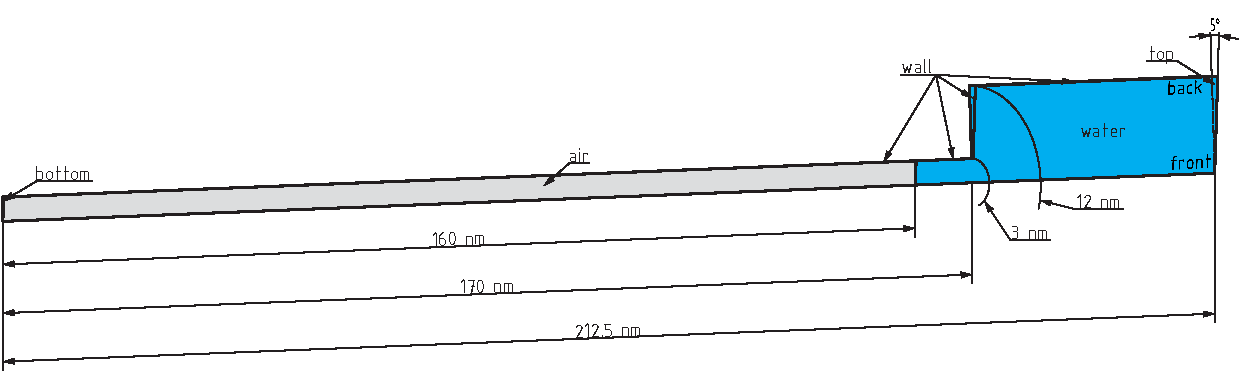
\includegraphics[width=.95\textwidth]{Pictures/Cap_5DEG.pdf}
    \caption{Schematic of used Capillary}
    \label{fig: Capillary Geometry}
\end{figure}
As already indicated in the picture, not the entire capillary is simulated, but only a segment of the capillary, called a \textit{wedge}. It is assumed that the flow in the capillary is axisymmetric, which greatly simplifies the simulation in that fewer elements are needed for discretization, as in this case only a $5^{\circ}$ segment of the capillary is simulated. A necessary condition for simulating the wedge is that it may only have one element in the radial direction. The discretization of the geometry was chosen so that the elements have an edge length of $0.2nm$. To create the \texttt{blockMeshDict} file, a python script was created that creates a file based on the capillary diameter and length with the designations of the surfaces shown in Figure \ref{fig: Capillary Geometry}.

\section{Boundary Conditions}
In Figure \ref{fig: Capillary Geometry}, in addition to the geometry, the surfaces that were provided with boundary conditions are also named. The \texttt{front} and \texttt{back} surfaces are opposing surfaces of the wedge and must therefore receive corresponding boundary conditions. The \texttt{wall} surfaces are impenetrable surfaces, and the \texttt{top} and \texttt{bottom} surfaces are surfaces through which a flow is permitted.
The essential boundary conditions on the wall are listed in Table \ref{tab: BoundaryConditions_wall}.

\begin{table}[h]
    \centering
    \caption{Relevant boundary conditions for the wall}
    \label{tab: BoundaryConditions_wall}
    \begin{tabular}{lll}
        Parameter & Value \\ \hline
        Order parameter $C$ & \texttt{equilibriumPhaseContactAngle} \\
        Equilibrium contact angle $\theta_{\mathrm{e}}$ & $15^{\circ}$, $45^{\circ}$, $75^{\circ}$ \\
        Chemical potential $\phi$ & \texttt{zeroGradient} \\
        Velocity $\mathbf{u}$ & $\mathbf{u_{\mathrm{w}}} = 0$ \\
        Pressure $p$ & \texttt{fixedFluxPressure} \\
    \end{tabular}
\end{table}
For the order parameter $C$, the equilibrium boundary condition is assumed, and the equilibrium contact angle for each of the three simulations with this geometry is given as $15^{\circ}$, $45^{\circ}$, and $75^{\circ}$. For further simulations, in addition to the mentioned equilibrium condition \texttt{equilibriumPhaseContactAngle}, it was also assumed that there is an imbalance according to \ref{sec: nonEquiBC}. For the simulations, the boundary condition must be changed to \texttt{outOfEquilibriumPhaseContactAngle}, and a value for $\Gamma_{\mathrm{w}}$ must be specified.
The gradient of the chemical potential on the wall is set to zero, as is the velocity of the wall. The boundary condition for the pressure is chosen with \texttt{fixedFluxPressure} so that the pressure gradient is adjusted in such a way that the mass flow at the boundary matches the given velocity on the wall.
At the inlet or outlet of the capillary, a \texttt{zeroGradient} boundary condition also applies, and a pressure of $0$ Pa.

\section{Material Properties}
For the simulation, water and air at $25^{\circ}$ Celsius are assumed as the medium, among other things. This results in the material properties shown in Table \ref{tab:physicalProperties_CaseSetup}.
\begin{table}[h]
    \centering
    \caption{Physical properties}
    \label{tab:physicalProperties_CaseSetup}
    \begin{tabular}{lll}
        Fluid & Density $\frac{kg}{m^3}$ & Kinematic viscosity $\frac{m^2}{s}$ \\ \hline
        Water & $1000$ & $1.00E-06$ \\
        Air & $1$ & $1.00E-05$ \\
    \end{tabular}
\end{table}
The surface tension for a water-air interface at $25^{\circ}$ Celsius is given as \(0.072 N/m\). The interface thickness \( \epsilon \) was chosen to be approximately \(1.7 nm\) \cite{bagheriInterfacialRelaxationCrucial2022}, corresponding to the physical interface thickness.


\section{Simulation Parameters}
The mobility ($\kappa$) is a factor in the phase-field simulation that is difficult to determine. Jacqmin \cite{jacqmin1999CalculationTwoPhaseNavier} suggested an asymptotic behavior for \( \kappa \) of 
\begin{equation}
    \kappa = \mathcal{O}(\epsilon^{\delta})
\end{equation}
and showed that \( 1 \leq \delta < 2 \). Unfortunately, there is currently no concrete method for calculating mobility. Therefore, various simulations were conducted to determine a suitable value. The same applies to the wall relaxation factor $\Gamma_{\mathrm{w}}$. The fact that these parameters are phenomenological makes their prediction challenging, and there are only recommendations available.
For this work, a value of \( \kappa = 1.6 \times 10^{-18} \) was used. For the wall relaxation factor $\Gamma_{\mathrm{w}}$, a value of \( \Gamma_{\mathrm{w}} = 5 \times 10^{12} \) was assumed. \todo{CHECK}

Due to initial problems in post-processing, the simulation was conducted without adaptive mesh refinement.
The simulation was initialized with a planar interface, and for the order parameter, an interface profile according to Equation \ref{eq: InterfactialNormalDirProfile} was initialized using the \texttt{funkySetFields} method.

The viscosity model of the simulation is carried out using the \texttt{blended} method. In this approach, the \texttt{arithmetic} and \texttt{harmonic} models are combined using a blending factor.


\section{Evaluation Methods}
For the evaluation of the simulation, the software \texttt{paraview} was used, among other tools. All images of the simulation were generated using this software. However, the evaluation and representation of derived or calculated quantities in diagrams were produced using the Python library \texttt{Matplotlib}. A script was developed to collect the results from the function objects and, if necessary, to perform calculations with them.

With the help of \textit{function objects}, data can be collected during the ongoing simulation. \texttt{phaseFieldFoam} provides several functions for reading out the simulation, which are also used here. These have to be integrated and configured in the \texttt{controlDict} file.

For instance, to analyze the viscous forces acting within the water column, we need the total viscous dissipation force in that water column, which is exported via such function objects. We obtain this by integrating the divergence of the viscous stress tensor $\tau$ from Equation \ref{eq: NSEChanged} over the domain:
\begin{equation}
    \mathrm{F}_{\mathrm{visc}}^{\mathrm{total}} = \int_{\Omega} \mathrm{f}_{\mathrm{visc}}^{\mathrm{total}} dV = \int_{\Omega} \nabla \cdot \tau dV.
\end{equation}



\chapter{Validation}
\label{chap: Validation}
The solver \texttt{phaseFieldFoam} has already been validated for various problems multiple times. Simulations with a wedge were also conducted with adaptive mesh refinement in \cite{holzinger2021DirectNumericalSimulation}. Simulations of capillaries or parallel plates were carried out in Hagg \cite{hagg2019DirekteNumerischeSimulation} and by Cai et al. \cite{cai2015NumericalSimulationWetting}. Samkhaniani et al. \cite{samkhaniani2021BouncingDropImpingement} simulated a bouncing droplet on a hydrophobic surface. Many other interesting and essential simulations and validations have been conducted with \texttt{phaseFieldFoam} \cite{bodziony2023StressfulWayDroplets,yinDirectNumericalSimulation,worner2021SpreadingReboundDynamics,bagheriInterfacialRelaxationCrucial2022}, whose individual mention would go beyond the scope of this work.
Since the solver has been validated in many places, only a Laplace test is conducted in this work. With Equation \ref{eq: YoungLaplaceEQ}, the pressure difference can be calculated for a settling radius of the simulation's interface and compared with the theoretical value. For this comparison, the radius of the interface in the simulation must be known. Assuming that the circle's center lies on the axis of rotation, the radius can be calculated using
\begin{equation}
    r_{\mathrm{S}} = \frac{R^2}{2h}+\frac{h}{2}
\end{equation}
\begin{figure}[h]
    \centering
    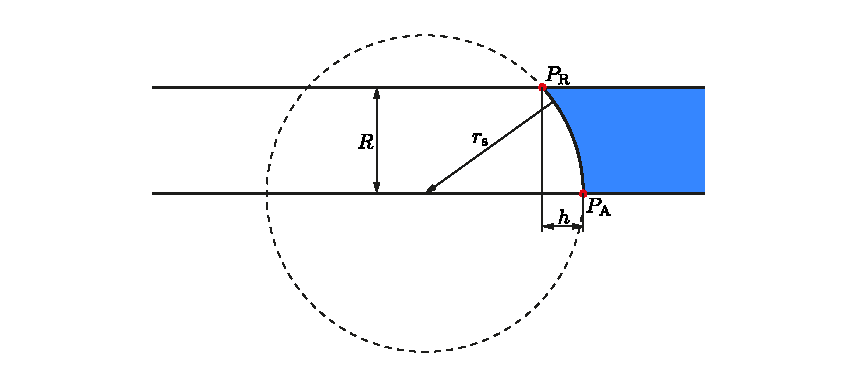
\includegraphics[width=.95\textwidth]{Pictures/RadiusCalc.pdf}
    \caption{Schematic of the capillary with relevant dimensions for the calculation of the radius}
    \label{fig: RadiusCalc}
\end{figure}

Figure \ref*{fig: RadiusCalc} shows the geometry of the capillary with the relevant dimensions. The points $P_{\mathrm{R}}$ and $P_{\mathrm{A}}$ are the intersection points of the interface with the capillary wall and the axis of rotation. If these points are known, the height $h$ of the spherical segment can be calculated, and thus the sphere's radius $r_{\mathrm{S}}$ with the already known capillary radius $R$. The dashed line is intended to clarify that the sphere's radius does not necessarily have to correspond to that of the capillary.


\chapter{Results}
\label{chap: Results}
\todo[inline]{The Position of the meniskus was exported with paraview in the decomposed state. The position was then extracted with a python script.Probe data was preprocessed as well and several computations for eval of simulations. Plots were generated with matplotlib?; Start of real results with an overview when what where. Maybe work with normalized data? }


Wie in Kapitel \ref{sec: capillaryRise} gezeigt, ist der Kapillare Aufstieg bis heute nicht verstanden. Ziel dieser Arbeit ist es daher 


Wie bereits beschrieben soll der Übergang vom linearen Anstieg der höhe einer Wassersäule in einer Kapillare hin zum Lucas Washburn Regime Untersucht werden. Weiter wurde beschrieben wie Delanoy et al. \cite{delannoy2019DualRoleViscosity} oder Ruiz et al. \cite{ruiz-gutierrez2022LongCrossoverDynamics} das Wachstum beschrieben. Zum Vergleich damit werden zunächst die Zeitpunkte oder Längen anhand ihrer vorhersagen berechnet und anschließend verglichen. Zunächst aber ein direkter Vergleich mit der Lucas-Washburn Gleichung. 
Delanoy et al. \cite{delannoy2019DualRoleViscosity} oder Ruiz et al. \cite{ruiz-gutierrez2022LongCrossoverDynamics} haben eigene Ansätze gefunden, um den Übergang zwischen den beiden Wachstumsregionen zu beschreiben. 


Im folgenden werden die Ergebnisse der Simulationen diskutiert und versucht eine Beschreibung für den Übergang der vorgestellten Wachstumsregionen des Kapillaren Aufstiegs zu finden. Um mögliche einflüsse durch den Kontaktwinkel berücksichtigen zu können wurden die Simulationen mit drei unterschiedlichen Kontaktwinkeln durchgeführt. Bei den verwendeten Dimensionen der Kapillare und der Flüssigkeiten, ist zu erwarten, dass der Einfluss der Gravitation vernachlässigbar ist, was auch in gesondert durchgeführten Simulationen gezeigt werden konnte, jedoch aufgrund der geringen aussagekraft eines Vergleichs mit Simulationen ohne Gravitation nicht weiter betrachtet wird. Damit wird jedoch auch klar, dass eine der besprochenen von Lucas und Washburn angenommen Vereinfachnungen für diesen Fall nicht gelten und eine Abweichung der vorhersage mit Gleichung \ref{eq: LW-Eq} darauf zurückzuführen ist, dass ein Gleichgewicht zwischen Kapillarkraft und viskosem drag nicht ausreicht, um den Kapillaren Aufstieg in frühen imbibitionsstadien zu beschreiben. 

Abbildung \ref{fig: LW-PFF_comp} zeigt einen direkten vergleich der Simulationsergebnisse mit der Lucas-Washburn Gleichung (rote linie \todo{describe as in actual figure later}). Darin wurde in \ref{fig: LW-PFF_comp} (a) linear skalliert und in \ref{fig: LW-PFF_comp} (b) logarithmisch. In der logarithmischen Darstellung werden die Unterschiede deutlich sichtbar. Zu Beginn ist die Steigung der Simulationen größer als die der vorhersage, bis sie sich schließlich annähern. Das lässt darauf schließen, dass der Kapillare Aufstieg erst nach einiger Zeit dem bekannten Lucas Washburn Wachstum folgt. Dies 

Wie ebenfalls bereits beschrieben sagt die Lucas-Washburn Gleichung ein Wachstum von $z(t)\sim \sqrt{t}$ vorher. 

\begin{figure}[h]
    \centering
    \includegraphics[width=.95\textwidth]{Pictures/LW-PFF_comp.png}
    \caption{Vergleich des von Lucas-Washburn vorhergesagten Wachstums mit den Ergenissen von \texttt{phaseFieldFoam}}
    \label{fig: LW-PFF_comp}
\end{figure}

\chapter{Outlook}
\label{chap: Outlook}
\begin{itemize}
    \item complex geometry
    \item temperature dependent capillary rise?
    \item surfactants and capillary rise?
    \item more fluids with other viscosisties
    \item in depth reseach of gamma value and possible dependence of mesh resolution
\end{itemize}

\printbibliography

\end{document}
